\documentclass[12pt]{article}
\usepackage{geometry}
\geometry{a4paper}
\usepackage{graphicx}

\begin{document}
\title{Human-Centered Design}
\author{James Simpson \and Alina Boghiu \and Amer Sinha \and Shahab Shirazi \and Jack Siebert}
\date{\today}
\maketitle

\section{Introduction}
The purpose of our research has been to design a product that will benefit members of the 50+ age group. After talking to family and friends we identified a problem, created a persona and focused on designing a product that is feasible, affordable and comfortable to use.

\section{Research}
In order to identify a problem we conducted research amongst our potential clients. We also considered existing resources and consulted several studies and statistics.

	\subsection{The People}
	The first people to approach were our family. This led to the creation of two personas.

	\begin{itemize}
	\item \textbf{Emilia} (54) is a mother. Her job as a teacher involves her in many scholar activities which keep her very active. Last year she was diagnosed with breast cancer for which she undertook surgery and chemotherapy. Currently she is fine but must take medication daily. She takes this very seriously but because of her busy lifestyle she keeps forgetting about it. It's never her main focus.

	\item \textbf{Gladys} (72) is a grandmother. blah blah blah
	\end{itemize}

	\subsection{The Problem}
	After talking to people about their problems it became obvious that medication is a very important part of their life. At the same time people don't pay much attention to it which leads to the issue we identified as our main focus:\medskip \\ \emph{People forget to take their medicine.} \medskip \\
	There are several reasons for this, ranging from being too busy (like Emilia) or too old to remember (like Gladys), to simply not being able to sort out the dosage or not regarding it as important etc.

	\subsection{Previous Studies}
	With this problem in mind we extended our research to include previous studies and statistics. This revealed several interesting facts:
	\begin{itemize}
	\item In the U.K. 45\% of medications are prescribed for people of age 75 and over and about half of those people do not take their medications as instructed. 
	\item In the U.S. 1 in 4 of individuals 65 years old and older take between 10 and 19 pills each day. Around 60\% of those admit that they either FORGET to take their medications or they forget doses. \footnote{Med Ad News February 2010}
	\item This rate of non-compliance is a worldwide problem just as dangerous and costly as an illness itself. The cost is estimated at £60 billion a year worldwide.
	\end{itemize}


\section{The Solution}
	\subsection{Current Solutions}
	Because the problem is clearly existent, none of the current solutions would prove satisfactory. Nevertheless it is important to study what about the current solutions is wrong.

	\begin{enumerate}
	\item \textbf{The Alarm Clock} - The patient can set a reminder on their phone or clock. \\ Problem: This does not ensure they will actually take the medication nor does it tell the patient which pill and how much to take. Emilia also had problems with remembering to set the actual alarm. More so, considering medications need to be taken at several times of the day, several alarms would need to be set and this can get very confusing.
	\item \textbf{The Medical Professional} - The patient can hire a medical assistant to come around the house and give them their medication. \\ Problem: This is a very expensive solution and often no trained personnel will be available to take this time consuming and tedious job. Gladys also is reluctant to letting strangers in her house so often and refused this solution completely.
	\item \textbf{The Pill Agenda} - The medication can be previously sorted by the pharmacist or doctor using the sistem in the following image. \\ Problem: This does not actually remind the patient to take the medication. It is Gladys is current system and it has happened more than once for her son to come and find the pills are untouched. This is a very serious situation because once missed, one cannot go back in time to take the prescribed dosage.
	\end{enumerate}

	\subsection{The Systems Approach}
	With this in mind we used the systems approach to come up with a device and thought of the inputs: we want to feed in the medication and dosage information, check if the patient has taken it and output accordingly. \\
	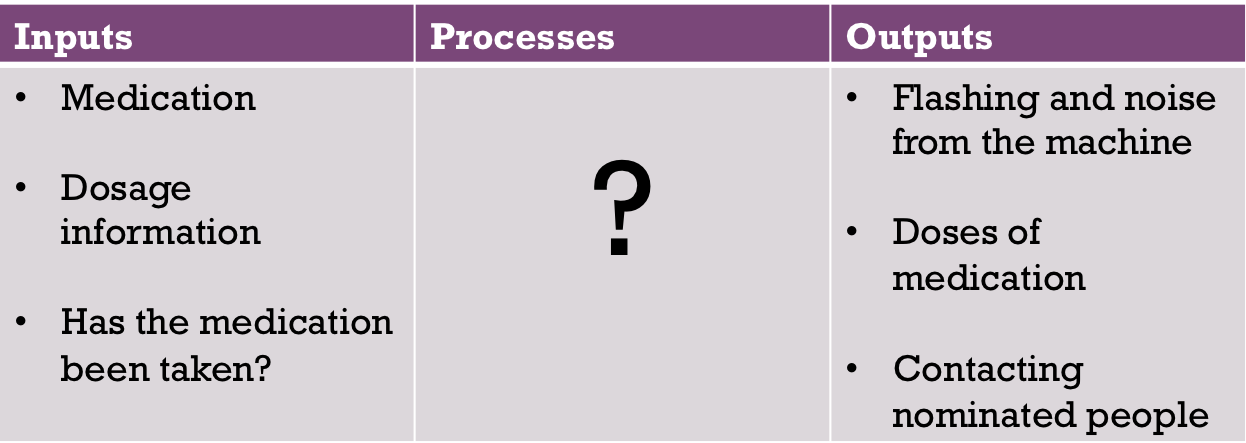
\includegraphics[width=\textwidth]{systems.png}
	When designing a product with these specifications we had one key feature in mind: \\ \emph{The patient should not have to know anything more than they already do} \\ Ideally, they would be fed the right pills at the right time in the right dosage. We wanted a solution similar to the second one described above (the medical professional) but without the cost or the inconvenience of having someone come into your home.\medskip\\

	\subsection{The product}
	Finally our product shaped up to be a coffe-machine-like pill dispenser. These are the first key features:
	\begin{itemize}
	\item Simplicity: no buttons or other interaction methods.
	\item Safty: the pharmacist sells pre-packed tubes of medication, with a chip that the machine can read and know how much and when to dispense. No one else has access to the dosage or content of the tubes.
	\item Reliability: The machine notifies the user until it detects that the dispensed medicine is no longer in the tray. After a certain delay it notifies the nominated responsible person. The machine also notifies about low supplies of pills.
	\item Low cost: Once purchased the patient only pays for the medication. The containers (tubes) can be reprogrammed.
	\end{itemize}
	With this in mind we sketched the physical product. These are a few attempts that focus on reduced size and pleasant aspect. \\
	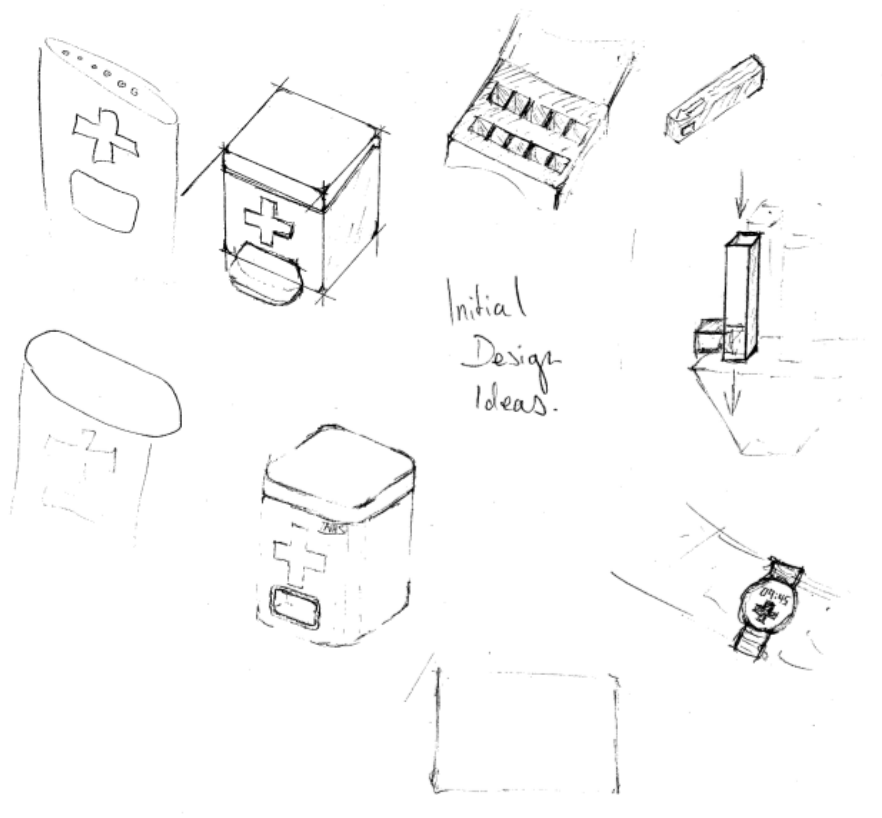
\includegraphics[width=0.85\textwidth]{product.png}

	\subsubsection*{How it works in detail}
	Description \\
	Programming the tubes - considering intermediate users \\
	Notifying the patient - from the bracelet to the telephone (working with and for the user)

	\subsection{Quantified self}
	\subsection{Value and Technical Feasibility}

\section{Summary}

\end{document}
